\documentclass[11pt, a4paper]{article}\usepackage[]{graphicx}\usepackage[]{xcolor}
% maxwidth is the original width if it is less than linewidth
% otherwise use linewidth (to make sure the graphics do not exceed the margin)
\makeatletter
\def\maxwidth{ %
  \ifdim\Gin@nat@width>\linewidth
    \linewidth
  \else
    \Gin@nat@width
  \fi
}
\makeatother

\definecolor{fgcolor}{rgb}{0.345, 0.345, 0.345}
\newcommand{\hlnum}[1]{\textcolor[rgb]{0.686,0.059,0.569}{#1}}%
\newcommand{\hlstr}[1]{\textcolor[rgb]{0.192,0.494,0.8}{#1}}%
\newcommand{\hlcom}[1]{\textcolor[rgb]{0.678,0.584,0.686}{\textit{#1}}}%
\newcommand{\hlopt}[1]{\textcolor[rgb]{0,0,0}{#1}}%
\newcommand{\hlstd}[1]{\textcolor[rgb]{0.345,0.345,0.345}{#1}}%
\newcommand{\hlkwa}[1]{\textcolor[rgb]{0.161,0.373,0.58}{\textbf{#1}}}%
\newcommand{\hlkwb}[1]{\textcolor[rgb]{0.69,0.353,0.396}{#1}}%
\newcommand{\hlkwc}[1]{\textcolor[rgb]{0.333,0.667,0.333}{#1}}%
\newcommand{\hlkwd}[1]{\textcolor[rgb]{0.737,0.353,0.396}{\textbf{#1}}}%
\let\hlipl\hlkwb

\usepackage{framed}
\makeatletter
\newenvironment{kframe}{%
 \def\at@end@of@kframe{}%
 \ifinner\ifhmode%
  \def\at@end@of@kframe{\end{minipage}}%
  \begin{minipage}{\columnwidth}%
 \fi\fi%
 \def\FrameCommand##1{\hskip\@totalleftmargin \hskip-\fboxsep
 \colorbox{shadecolor}{##1}\hskip-\fboxsep
     % There is no \\@totalrightmargin, so:
     \hskip-\linewidth \hskip-\@totalleftmargin \hskip\columnwidth}%
 \MakeFramed {\advance\hsize-\width
   \@totalleftmargin\z@ \linewidth\hsize
   \@setminipage}}%
 {\par\unskip\endMakeFramed%
 \at@end@of@kframe}
\makeatother

\definecolor{shadecolor}{rgb}{.97, .97, .97}
\definecolor{messagecolor}{rgb}{0, 0, 0}
\definecolor{warningcolor}{rgb}{1, 0, 1}
\definecolor{errorcolor}{rgb}{1, 0, 0}
\newenvironment{knitrout}{}{} % an empty environment to be redefined in TeX

\usepackage{alltt}

\usepackage[top=1 in, bottom = 1 in, left = 1 in, right = 1 in ]{geometry}

\usepackage{amsmath, amssymb, amsfonts}
\usepackage{enumerate}

\title{Two-way ANOVA - m observations per cell - fixed effects model}
\author{Ananda Biswas}
\date{}
\IfFileExists{upquote.sty}{\usepackage{upquote}}{}
\begin{document}

\maketitle



\begin{knitrout}
\definecolor{shadecolor}{rgb}{0.969, 0.969, 0.969}\color{fgcolor}\begin{kframe}
\begin{alltt}
\hlstd{birth_weight_data} \hlkwb{<-} \hlkwd{read.csv}\hlstd{(}\hlstr{"D:\textbackslash{}\textbackslash{}data_sets\textbackslash{}\textbackslash{}birth-weight.csv"}\hlstd{,}
    \hlkwc{stringsAsFactors} \hlstd{=} \hlnum{TRUE}\hlstd{)}
\end{alltt}
\end{kframe}
\end{knitrout}

\section*{Loading the dataset and having a first look at it}

\begin{knitrout}
\definecolor{shadecolor}{rgb}{0.969, 0.969, 0.969}\color{fgcolor}\begin{kframe}
\begin{alltt}
\hlstd{birth_weight_data}
\end{alltt}
\begin{verbatim}
##    order_of_gravida age.group_of_mother birth.weight_of_babies
## 1                 1               15-20                    5.1
## 2                 1               15-20                    5.0
## 3                 1               15-20                    4.8
## 4                 1               20-25                    5.0
## 5                 1               20-25                    5.1
## 6                 1               20-25                    5.3
## 7                 1               25-30                    5.1
## 8                 1               25-30                    5.1
## 9                 1               25-30                    4.9
## 10                1               30-35                    4.9
## 11                1               30-35                    4.9
## 12                1               30-35                    5.0
## 13                1         35 and over                    5.0
## 14                1         35 and over                    5.0
## 15                1         35 and over                    5.0
## 16                2               15-20                    5.2
## 17                2               15-20                    5.2
## 18                2               15-20                    5.4
## 19                2               20-25                    5.3
## 20                2               20-25                    5.3
## 21                2               20-25                    5.5
## 22                2               25-30                    5.3
## 23                2               25-30                    5.2
## 24                2               25-30                    5.2
## 25                2               30-35                    5.2
## 26                2               30-35                    5.0
## 27                2               30-35                    5.5
## 28                2         35 and over                    5.1
## 29                2         35 and over                    5.3
## 30                2         35 and over                    5.0
## 31                3               15-20                    5.8
## 32                3               15-20                    5.7
## 33                3               15-20                    5.9
## 34                3               20-25                    6.0
## 35                3               20-25                    5.9
## 36                3               20-25                    6.2
## 37                3               25-30                    5.8
## 38                3               25-30                    5.9
## 39                3               25-30                    5.9
## 40                3               30-35                    5.8
## 41                3               30-35                    5.5
## 42                3               30-35                    5.5
## 43                3         35 and over                    5.9
## 44                3         35 and over                    5.4
## 45                3         35 and over                    5.5
## 46                4               15-20                    6.0
## 47                4               15-20                    6.0
## 48                4               15-20                    5.9
## 49                4               20-25                    6.2
## 50                4               20-25                    6.5
## 51                4               20-25                    6.0
## 52                4               25-30                    6.0
## 53                4               25-30                    6.1
## 54                4               25-30                    6.0
## 55                4               30-35                    6.0
## 56                4               30-35                    5.8
## 57                4               30-35                    5.5
## 58                4         35 and over                    5.8
## 59                4         35 and over                    5.6
## 60                4         35 and over                    5.5
## 61       5 and over               15-20                    6.0
## 62       5 and over               15-20                    6.0
## 63       5 and over               15-20                    6.0
## 64       5 and over               20-25                    6.0
## 65       5 and over               20-25                    6.1
## 66       5 and over               20-25                    6.3
## 67       5 and over               25-30                    5.9
## 68       5 and over               25-30                    6.0
## 69       5 and over               25-30                    5.8
## 70       5 and over               30-35                    5.9
## 71       5 and over               30-35                    6.0
## 72       5 and over               30-35                    5.5
## 73       5 and over         35 and over                    5.5
## 74       5 and over         35 and over                    6.0
## 75       5 and over         35 and over                    6.2
\end{verbatim}
\end{kframe}
\end{knitrout}

\begin{knitrout}
\definecolor{shadecolor}{rgb}{0.969, 0.969, 0.969}\color{fgcolor}\begin{kframe}
\begin{alltt}
\hlkwd{dim}\hlstd{(birth_weight_data)}
\end{alltt}
\begin{verbatim}
## [1] 75  3
\end{verbatim}
\end{kframe}
\end{knitrout}

\begin{knitrout}
\definecolor{shadecolor}{rgb}{0.969, 0.969, 0.969}\color{fgcolor}\begin{kframe}
\begin{alltt}
\hlkwd{names}\hlstd{(birth_weight_data)}
\end{alltt}
\begin{verbatim}
## [1] "order_of_gravida"       "age.group_of_mother"    "birth.weight_of_babies"
\end{verbatim}
\end{kframe}
\end{knitrout}

\begin{knitrout}
\definecolor{shadecolor}{rgb}{0.969, 0.969, 0.969}\color{fgcolor}\begin{kframe}
\begin{alltt}
\hlkwd{head}\hlstd{(birth_weight_data)}
\end{alltt}
\begin{verbatim}
##   order_of_gravida age.group_of_mother birth.weight_of_babies
## 1                1               15-20                    5.1
## 2                1               15-20                    5.0
## 3                1               15-20                    4.8
## 4                1               20-25                    5.0
## 5                1               20-25                    5.1
## 6                1               20-25                    5.3
\end{verbatim}
\end{kframe}
\end{knitrout}

\begin{knitrout}
\definecolor{shadecolor}{rgb}{0.969, 0.969, 0.969}\color{fgcolor}\begin{kframe}
\begin{alltt}
\hlkwd{tail}\hlstd{(birth_weight_data)}
\end{alltt}
\begin{verbatim}
##    order_of_gravida age.group_of_mother birth.weight_of_babies
## 70       5 and over               30-35                    5.9
## 71       5 and over               30-35                    6.0
## 72       5 and over               30-35                    5.5
## 73       5 and over         35 and over                    5.5
## 74       5 and over         35 and over                    6.0
## 75       5 and over         35 and over                    6.2
\end{verbatim}
\end{kframe}
\end{knitrout}

\begin{knitrout}
\definecolor{shadecolor}{rgb}{0.969, 0.969, 0.969}\color{fgcolor}\begin{kframe}
\begin{alltt}
\hlkwd{library}\hlstd{(tidyverse)}
\end{alltt}


{\ttfamily\noindent\color{warningcolor}{\#\# Warning: package 'tidyverse' was built under R version 4.2.3}}

{\ttfamily\noindent\color{warningcolor}{\#\# Warning: package 'ggplot2' was built under R version 4.2.2}}

{\ttfamily\noindent\color{warningcolor}{\#\# Warning: package 'tibble' was built under R version 4.2.3}}

{\ttfamily\noindent\color{warningcolor}{\#\# Warning: package 'tidyr' was built under R version 4.2.3}}

{\ttfamily\noindent\color{warningcolor}{\#\# Warning: package 'readr' was built under R version 4.2.2}}

{\ttfamily\noindent\color{warningcolor}{\#\# Warning: package 'purrr' was built under R version 4.2.3}}

{\ttfamily\noindent\color{warningcolor}{\#\# Warning: package 'dplyr' was built under R version 4.2.3}}

{\ttfamily\noindent\color{warningcolor}{\#\# Warning: package 'stringr' was built under R version 4.2.3}}

{\ttfamily\noindent\color{warningcolor}{\#\# Warning: package 'forcats' was built under R version 4.2.2}}

{\ttfamily\noindent\color{warningcolor}{\#\# Warning: package 'lubridate' was built under R version 4.2.2}}

{\ttfamily\noindent\itshape\color{messagecolor}{\#\# -- Attaching core tidyverse packages ------------------------ tidyverse 2.0.0 --\\\#\# v dplyr \ \ \ \ 1.1.3 \ \ \ \ v readr \ \ \ \ 2.1.4\\\#\# v forcats \ \ 1.0.0 \ \ \ \ v stringr \ \ 1.5.0\\\#\# v ggplot2 \ \ 3.4.1 \ \ \ \ v tibble \ \ \ 3.2.1\\\#\# v lubridate 1.9.2 \ \ \ \ v tidyr \ \ \ \ 1.3.0\\\#\# v purrr \ \ \ \ 1.0.2 \ \ \ \ \\\#\# -- Conflicts ------------------------------------------ tidyverse\_conflicts() --\\\#\# x dplyr::filter() masks stats::filter()\\\#\# x dplyr::lag() \ \ \ masks stats::lag()\\\#\# i Use the conflicted package (<http://conflicted.r-lib.org/>) to force all conflicts to become errors}}\end{kframe}
\end{knitrout}

\begin{knitrout}
\definecolor{shadecolor}{rgb}{0.969, 0.969, 0.969}\color{fgcolor}\begin{kframe}
\begin{alltt}
\hlstd{birth_weight_data} \hlopt
    \hlkwd{ggplot}\hlstd{(}\hlkwd{aes}\hlstd{(}\hlkwc{x} \hlstd{= order_of_gravida,}
        \hlkwc{y} \hlstd{= birth.weight_of_babies))} \hlopt{+}
    \hlkwd{stat_boxplot}\hlstd{(}\hlkwc{geom} \hlstd{=} \hlstr{"errorbar"}\hlstd{,}
        \hlkwc{linewidth} \hlstd{=} \hlnum{1}\hlstd{)} \hlopt{+} \hlkwd{geom_boxplot}\hlstd{(}\hlkwc{fill} \hlstd{=} \hlstr{"#7AEC34"}\hlstd{)} \hlopt{+}
    \hlkwd{labs}\hlstd{(}\hlkwc{x} \hlstd{=} \hlstr{"Order of Gravida"}\hlstd{,}
        \hlkwc{y} \hlstd{=} \hlstr{"Birth-weight of Babies"}\hlstd{,}
        \hlkwc{title} \hlstd{=} \hlstr{"Boxplot of Order of Gravida and Birth-weight of Babies"}\hlstd{)}
\end{alltt}
\end{kframe}
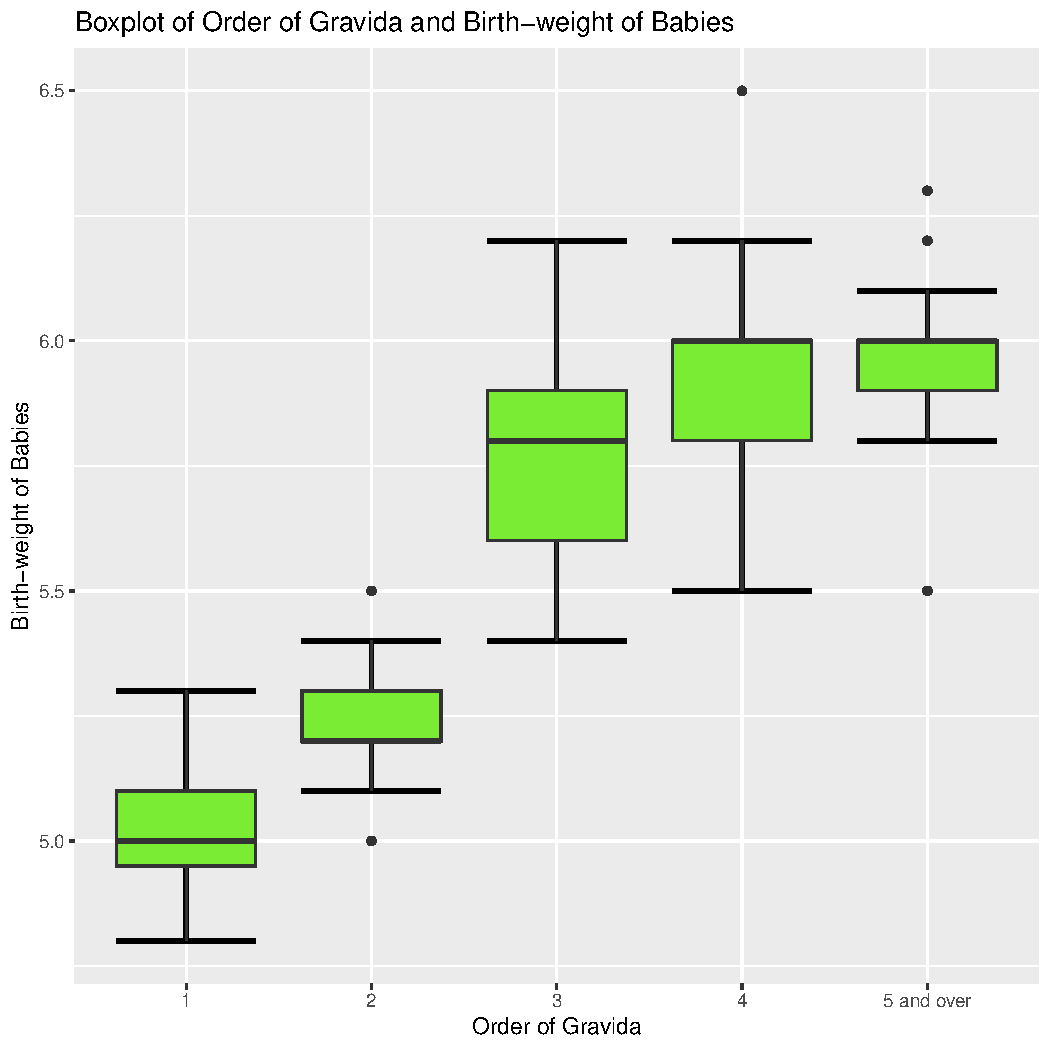
\includegraphics[width=\maxwidth]{figure/unnamed-chunk-8-1} 
\end{knitrout}

\newpage

\begin{knitrout}
\definecolor{shadecolor}{rgb}{0.969, 0.969, 0.969}\color{fgcolor}\begin{kframe}
\begin{alltt}
\hlstd{birth_weight_data} \hlopt
    \hlkwd{ggplot}\hlstd{(}\hlkwd{aes}\hlstd{(}\hlkwc{x} \hlstd{= age.group_of_mother,}
        \hlkwc{y} \hlstd{= birth.weight_of_babies))} \hlopt{+}
    \hlkwd{stat_boxplot}\hlstd{(}\hlkwc{geom} \hlstd{=} \hlstr{"errorbar"}\hlstd{,}
        \hlkwc{linewidth} \hlstd{=} \hlnum{1}\hlstd{)} \hlopt{+} \hlkwd{geom_boxplot}\hlstd{(}\hlkwc{fill} \hlstd{=} \hlstr{"#44F6E3"}\hlstd{)} \hlopt{+}
    \hlkwd{labs}\hlstd{(}\hlkwc{x} \hlstd{=} \hlstr{"Age-group of Mother"}\hlstd{,}
        \hlkwc{y} \hlstd{=} \hlstr{"Birth-weight of Babies"}\hlstd{,}
        \hlkwc{title} \hlstd{=} \hlstr{"Boxplot of Age-group of Mother and Birth-weight of Babies"}\hlstd{)}
\end{alltt}
\end{kframe}
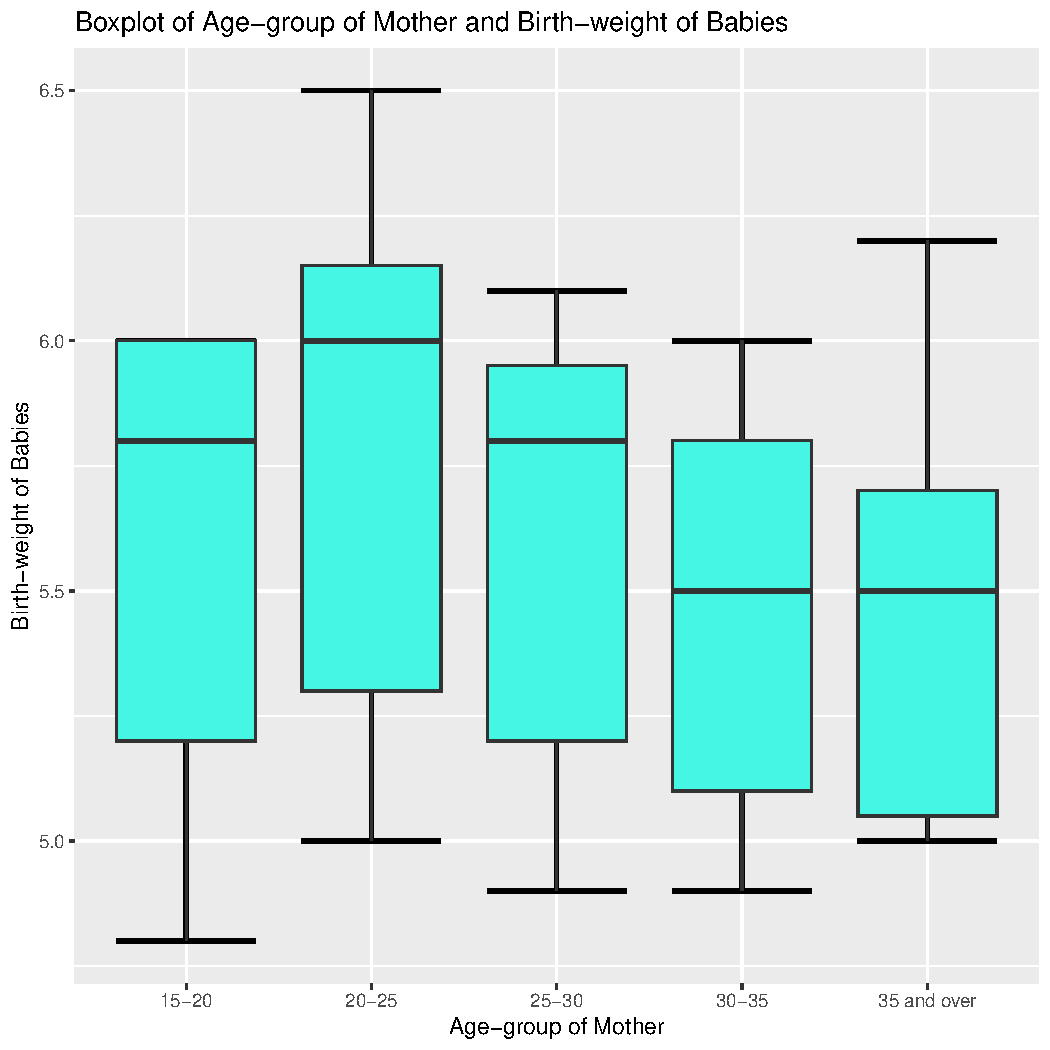
\includegraphics[width=\maxwidth]{figure/unnamed-chunk-9-1} 
\end{knitrout}


\newpage

\begin{knitrout}
\definecolor{shadecolor}{rgb}{0.969, 0.969, 0.969}\color{fgcolor}\begin{kframe}
\begin{alltt}
\hlstd{df1} \hlkwb{<-} \hlstd{birth_weight_data} \hlopt
    \hlkwd{group_by}\hlstd{(order_of_gravida,}
        \hlstd{age.group_of_mother)} \hlopt
    \hlkwd{summarise}\hlstd{(}\hlkwc{average_birth_weight} \hlstd{=} \hlkwd{mean}\hlstd{(birth.weight_of_babies))}
\end{alltt}


{\ttfamily\noindent\itshape\color{messagecolor}{\#\# `summarise()` has grouped output by 'order\_of\_gravida'. You can override using\\\#\# the `.groups` argument.}}\begin{alltt}
\hlstd{df1} \hlopt
    \hlkwd{ggplot}\hlstd{(}\hlkwd{aes}\hlstd{(}\hlkwc{x} \hlstd{= order_of_gravida,}
        \hlkwc{y} \hlstd{= average_birth_weight))} \hlopt{+}
    \hlkwd{geom_line}\hlstd{(}\hlkwd{aes}\hlstd{(}\hlkwc{group} \hlstd{= age.group_of_mother,}
        \hlkwc{color} \hlstd{= age.group_of_mother),}
        \hlkwc{linewidth} \hlstd{=} \hlnum{1.3}\hlstd{)} \hlopt{+} \hlkwd{geom_point}\hlstd{(}\hlkwd{aes}\hlstd{(}\hlkwc{color} \hlstd{= age.group_of_mother),}
    \hlkwc{size} \hlstd{=} \hlnum{3}\hlstd{)} \hlopt{+} \hlkwd{labs}\hlstd{(}\hlkwc{x} \hlstd{=} \hlstr{"Order of Gravida"}\hlstd{,}
    \hlkwc{y} \hlstd{=} \hlstr{"Average Birth-weight of Babies"}\hlstd{,}
    \hlkwc{title} \hlstd{=} \hlstr{"Interaction plot of Different age-groups of Mothers"}\hlstd{)}
\end{alltt}
\end{kframe}
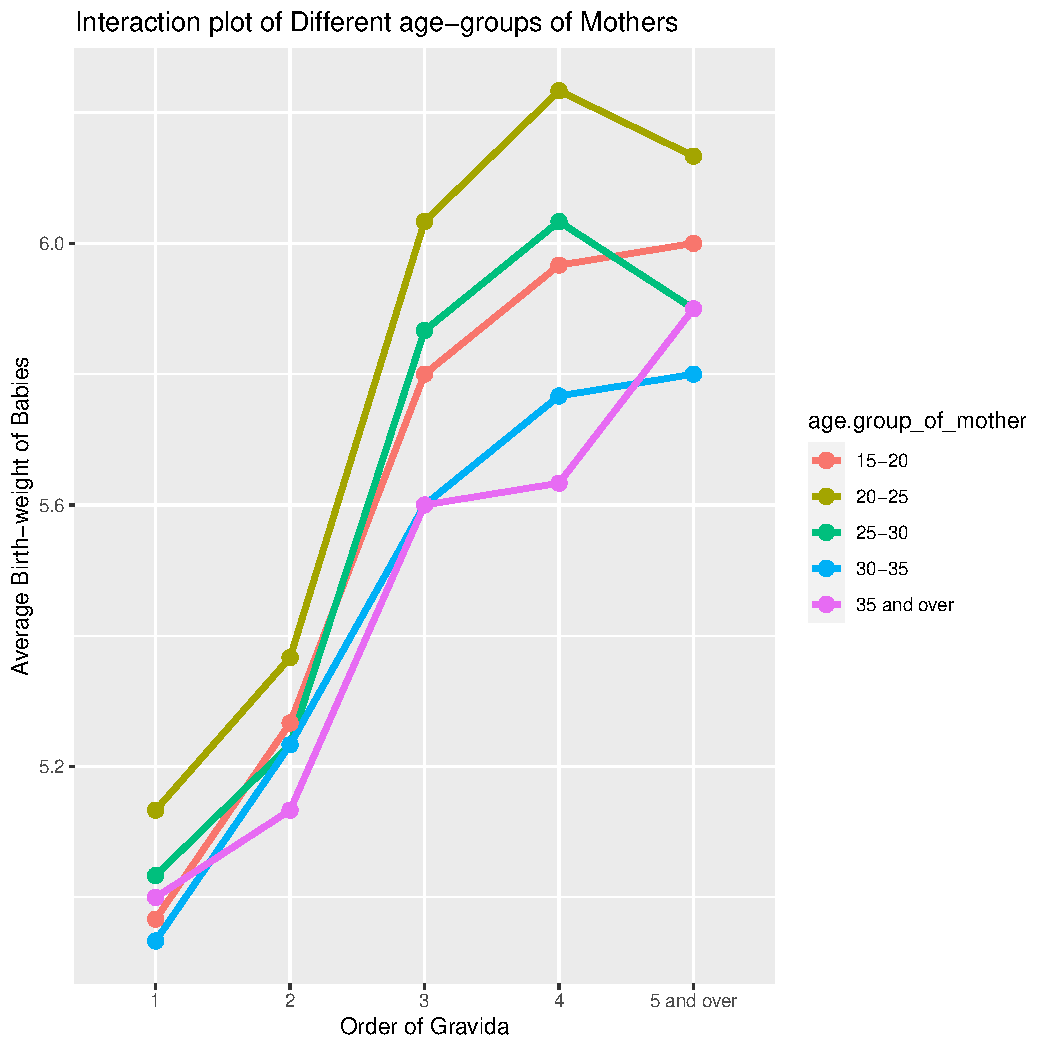
\includegraphics[width=\maxwidth]{figure/unnamed-chunk-10-1} 
\end{knitrout}


\begin{knitrout}
\definecolor{shadecolor}{rgb}{0.969, 0.969, 0.969}\color{fgcolor}\begin{kframe}
\begin{alltt}
\hlstd{birth_weight_anova} \hlkwb{<-} \hlkwd{aov}\hlstd{(birth.weight_of_babies} \hlopt{~}
    \hlstd{order_of_gravida} \hlopt{+} \hlstd{age.group_of_mother} \hlopt{+}
        \hlstd{order_of_gravida}\hlopt{:}\hlstd{age.group_of_mother,}
    \hlkwc{data} \hlstd{= birth_weight_data)}
\end{alltt}
\end{kframe}
\end{knitrout}

\begin{knitrout}
\definecolor{shadecolor}{rgb}{0.969, 0.969, 0.969}\color{fgcolor}\begin{kframe}
\begin{alltt}
\hlkwd{summary}\hlstd{(birth_weight_anova)}
\end{alltt}
\begin{verbatim}
##                                      Df Sum Sq Mean Sq F value   Pr(>F)    
## order_of_gravida                      4 10.902  2.7255  96.422  < 2e-16 ***
## age.group_of_mother                   4  1.055  0.2639   9.335 1.03e-05 ***
## order_of_gravida:age.group_of_mother 16  0.357  0.0223   0.788    0.691    
## Residuals                            50  1.413  0.0283                     
## ---
## Signif. codes:  0 '***' 0.001 '**' 0.01 '*' 0.05 '.' 0.1 ' ' 1
\end{verbatim}
\end{kframe}
\end{knitrout}

We see that the interaction effect due to order of gravida and age-group of mother is not significant. But the order of gravida and age-group of mother both significantly affect the birth-weight of the baby. \\


Now we consider a linear statistical model :

$$y_{ij} = \mu + \alpha_i + \beta_j + e_{ij} \,\, ; \,\,\,\, i = 1(1)5, j = 1(1)5$$

where $\mu$ is the average birth-weight of babies, \\
$\alpha_i$ is the additional birth-weight due to $i-th$ order of gravida, \\
$\beta_j$ is the additional birth-weight due to $j-th$ age-group of mother and \\
$e_{ij}$ is the random error. \\



Now we shall estimate the model parameters.

\begin{knitrout}
\definecolor{shadecolor}{rgb}{0.969, 0.969, 0.969}\color{fgcolor}\begin{kframe}
\begin{alltt}
\hlstd{fit1} \hlkwb{<-} \hlkwd{lm}\hlstd{(birth.weight_of_babies} \hlopt{~}
    \hlstd{order_of_gravida} \hlopt{+} \hlstd{age.group_of_mother,}
    \hlkwc{data} \hlstd{= birth_weight_data)}
\end{alltt}
\end{kframe}
\end{knitrout}

\begin{knitrout}
\definecolor{shadecolor}{rgb}{0.969, 0.969, 0.969}\color{fgcolor}\begin{kframe}
\begin{alltt}
\hlkwd{summary}\hlstd{(fit1)}
\end{alltt}
\begin{verbatim}
## 
## Call:
## lm(formula = birth.weight_of_babies ~ order_of_gravida + age.group_of_mother, 
##     data = birth_weight_data)
## 
## Residuals:
##      Min       1Q   Median       3Q      Max 
## -0.33067 -0.11400  0.02267  0.08933  0.38267 
## 
## Coefficients:
##                                Estimate Std. Error t value Pr(>|t|)    
## (Intercept)                     5.03067    0.05673  88.682  < 2e-16 ***
## order_of_gravida2               0.23333    0.05980   3.902 0.000226 ***
## order_of_gravida3               0.76667    0.05980  12.822  < 2e-16 ***
## order_of_gravida4               0.91333    0.05980  15.274  < 2e-16 ***
## order_of_gravida5 and over      0.93333    0.05980  15.609  < 2e-16 ***
## age.group_of_mother20-25        0.18000    0.05980   3.010 0.003695 ** 
## age.group_of_mother25-30        0.01333    0.05980   0.223 0.824238    
## age.group_of_mother30-35       -0.13333    0.05980  -2.230 0.029166 *  
## age.group_of_mother35 and over -0.14667    0.05980  -2.453 0.016825 *  
## ---
## Signif. codes:  0 '***' 0.001 '**' 0.01 '*' 0.05 '.' 0.1 ' ' 1
## 
## Residual standard error: 0.1638 on 66 degrees of freedom
## Multiple R-squared:  0.8711,	Adjusted R-squared:  0.8554 
## F-statistic: 55.74 on 8 and 66 DF,  p-value: < 2.2e-16
\end{verbatim}
\end{kframe}
\end{knitrout}

\begin{knitrout}
\definecolor{shadecolor}{rgb}{0.969, 0.969, 0.969}\color{fgcolor}\begin{kframe}
\begin{alltt}
\hlstd{fit1}\hlopt{$}\hlstd{rank}
\end{alltt}
\begin{verbatim}
## [1] 9
\end{verbatim}
\end{kframe}
\end{knitrout}

As the rank of the design matrix is 9, only 9 parameters are estimated. \\

The estimates of \textit{orderofgravida1} and \textit{agegroupofmotehr15-20} have been forced to 0.

\newpage

\begin{knitrout}
\definecolor{shadecolor}{rgb}{0.969, 0.969, 0.969}\color{fgcolor}\begin{kframe}
\begin{alltt}
\hlstd{temp_df} \hlkwb{<-} \hlkwd{data.frame}\hlstd{(fit1}\hlopt{$}\hlstd{residuals)}

\hlstd{temp_df} \hlopt
    \hlkwd{ggplot}\hlstd{(}\hlkwd{aes}\hlstd{(}\hlkwc{y} \hlstd{= fit1.residuals,}
        \hlkwc{x} \hlstd{=} \hlnum{1}\hlopt{:}\hlkwd{length}\hlstd{(fit1.residuals)))} \hlopt{+}
    \hlkwd{geom_point}\hlstd{(}\hlkwc{color} \hlstd{=} \hlstr{"red"}\hlstd{,} \hlkwc{size} \hlstd{=} \hlnum{1.5}\hlstd{)} \hlopt{+}
    \hlkwd{geom_hline}\hlstd{(}\hlkwc{yintercept} \hlstd{=} \hlnum{0}\hlstd{,}
        \hlkwc{col} \hlstd{=} \hlstr{"blue"}\hlstd{,} \hlkwc{linewidth} \hlstd{=} \hlnum{1}\hlstd{)} \hlopt{+}
    \hlkwd{labs}\hlstd{(}\hlkwc{x} \hlstd{=} \hlstr{"Index"}\hlstd{,} \hlkwc{y} \hlstd{=} \hlstr{"Residuals"}\hlstd{,}
        \hlkwc{title} \hlstd{=} \hlstr{"Residual Plot"}\hlstd{)}
\end{alltt}
\end{kframe}
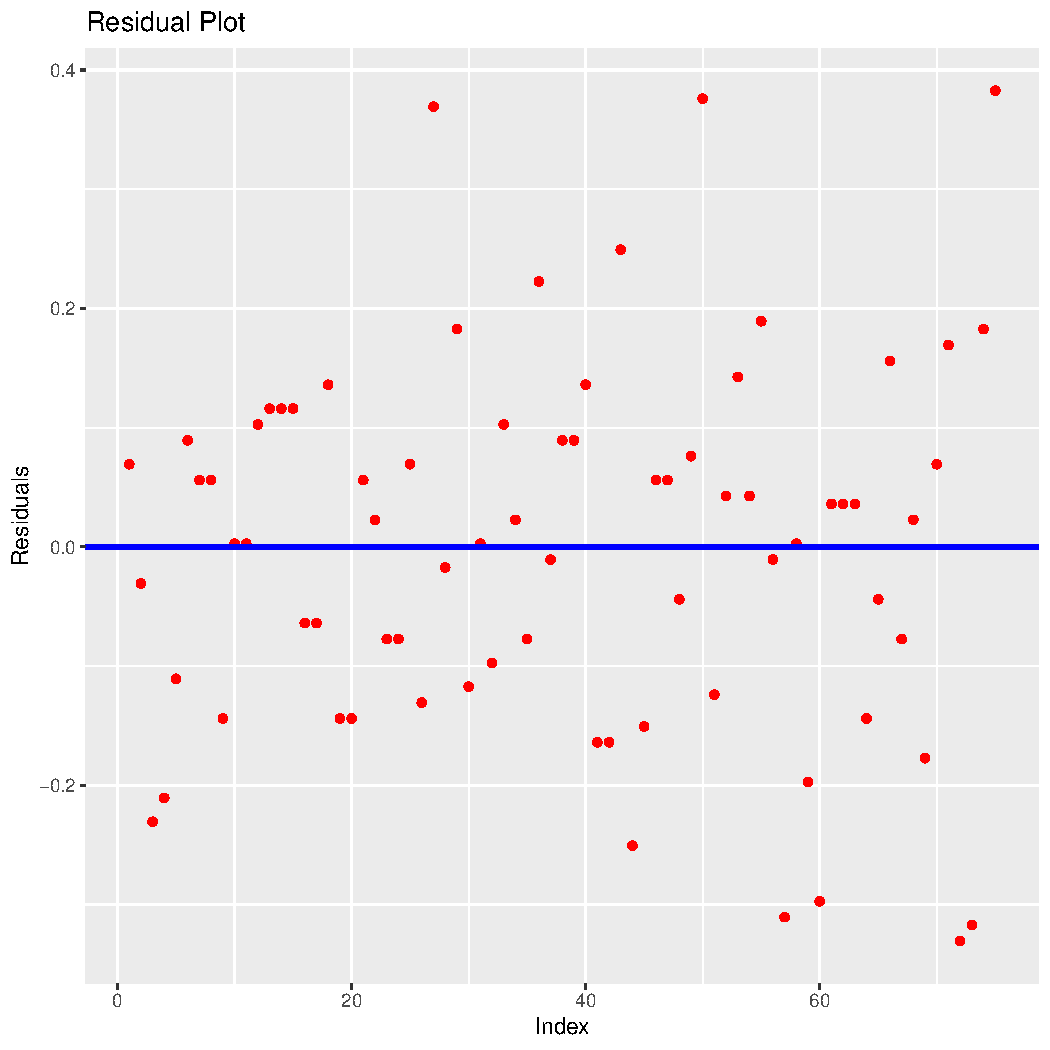
\includegraphics[width=\maxwidth]{figure/unnamed-chunk-16-1} 
\end{knitrout}

\end{document}
